\documentclass[12pt]{article}
\usepackage[pdftex]{graphicx}

\usepackage{qtree}

\usepackage{mathptmx}% http://ctan.org/pkg/mathptmx
\usepackage{times}
\usepackage{amsmath}
\usepackage{amsthm}
 \usepackage{amsfonts}
\theoremstyle{definition}
\newtheorem{definition}{Definition}[section]
\newtheorem{lemma}{Lemma}[section]


\title{People who want to parse bigrams and finite state machines\\good}
\author{Meaghan ``geitje'' Fowlie and Floris ``konijntje'' van Vugt}


\begin{document}

\maketitle

\section{Definitions}

%\newcommand\STATES{\mathcal{S}}
\newcommand\STATES{\ensuremath{\mathbb{S}}}
%\newcommand\OPS{\mathcal{O}}
\newcommand\OPS{\ensuremath{\mathbb{O}}}
%\newcommand\BIGR{\mathcal{B}}
\newcommand\BIGR{\ensuremath{\mathbb{B}}}
\newcommand\FSA{\textsc{FSA}}
%\newcommand\PARSES{\mathcal{P}}
\newcommand\PARSES{\ensuremath{\mathbb{P}}}
\newcommand\SC{\text{\textsc{sc}}}
\newcommand\TC{\text{\textsc{tc}}}
\newcommand\UC{\text{\textsc{uc}}}
\newcommand\BC{\text{\textsc{bc}}}
\newcommand\N{\ensuremath{\mathbb{N}}}
\newcommand\sg{\ensuremath{\Sigma}}
\newcommand\la{\ensuremath{\langle}}
\newcommand\ra{\ensuremath{\rangle}}
\newcommand\arr{\ensuremath{\rightarrow}}
\newcommand\emp{\ensuremath{\epsilon}}
\newcommand\op{\text{\textsl{op}}}
\newcommand\mg{\text{\textsl{mg}}}
\newcommand\cp{\text{\textsl{copy}}}
\newcommand\cl{\text{\textsl{clear}}}
\newcommand\ed{\text{\textsl{end}}}
\newcommand\expr{\text{\textsl{expr}}}
\newcommand\Lex{\text{\textsl{Lex}}}
\newcommand\fea[1]{\text{\texttt{#1}}}


\newcommand\der{\leftarrow}
%\newcommand\der{\text{:-}}


We define a deterministic finite state automaton over operations and a Markov chain over the alphabet. these two components make up the grammar. \\

\noindent\textbf{Notation} the size of a set or sequence $A$ is notated $|A|$ or $\#A$. The \textit{i}th member of a sequence $A$ is notated $A(i)$ and the last member $A(-1)$. $\epsilon$ is the empty sequence.


\subsection{The Grammar}
\label{sec:grammar}



\begin{definition}[Deterministic Finite State Automaton]
  A deterministic finite state automaton (DFSA) is a five-tuple 
\[\la \sg, Q, q_0, F, \delta  \ra  \]
where:

\noindent $\sg$ is an alphabet\\
$Q$ is a finite set (\textit{states})\\
$q_0\in Q$ is the designated \textit{start state}\\
$F\subseteq Q$ is the set of \textit{final states}\\
$\delta: Q\times \sg \arr Q$ is the \textit{transition function} 

A string $s\in\sg^*$ is accepted/generated by a DFSA $A$ iff
$\exists \mathbf{q} \in Q_A^*$ such that $\mathbf{q}(0)=q_0$, $\mathbf{q}(|\mathbf{q}|)\in F_A$, and $\forall i<|s|$, $\delta(\mathbf{q}(i),s(i))=\mathbf{q}(i+1)$
\label{def:dfsa}
\end{definition}

\begin{definition}
  We say a triple $(q,e,q')$ where $q,q'\in Q$ and $e\in\sg$ is a \textit{transition} of an
  FSA iff $\delta(q,e)=q'$.
\end{definition}

In our operations FSA, the set of all possible states is $\STATES$ and the alphabet is the set of all operations is $\OPS$. The bigram set or transition set, is $\BIGR$.


\begin{definition}[Operations FSA]
  The operations FSA is a deterministic finite state automaton over states \STATES~ and alphabet \OPS.
\end{definition}

\begin{definition}[Transition Probabilities]
   
  A probability assignment $\phi$ is a function from transitions of the operations FSA to [0,1] such that

$$\forall q\in \STATES,~~\sum_{e\in\OPS,q'\in \STATES} \phi(q,e,q') = 1 $$

\end{definition}

\begin{definition}[Markov Chain]
  A Markov chain is a 4-tuple $\la \sg, S, B, \phi  \ra $ where 

\sg~ is a finite alphabet of symbols, 

$S\subseteq \sg$ is a set of start categories,
 
$B\subseteq \sg\times\sg$ is a set of transitions between members of \sg, and

$\phi: \sg \times \sg \arr [0,1]$ is a probability distribution over transitions such that

$$\forall a\in \sg,~~\sum_{b\in\sg} \phi(a,b) = 1 $$


A sequence $s$ is accepted/generated by the chain iff $s$ is a sequence of alphabet items such that $s(0) \in S$ and $\forall i<|s|$, $(s(i),s(i+1))\in B$ 

\end{definition}

\begin{definition}[route]
  A \emph{route} is a route through the $\FSA$ of say $n$ steps, defined as a tuple $(Q,E)$ where $Q$ is the sequence of states visited, i.e.
%  $Q=\la q_i\in\STATES|i<n\ra$, and $E$ is the sequence of emissions.
 $E=\la e_i\in\OPS|i<n-1\ra$ such that $\forall i<n,~ \delta(q_i,e_i)=q_{i+1}$.

\end{definition}

  I think we need a homomorphism of the sort in Koller's paper to define the relationship between the operations and the surface strings?

\begin{definition}[expression]
  An expression is anything that can participate in an operation, i.e. for a given grammar over \sg:

  \expr = $(\sg^*\times\sg^*) \cup \sg^* \cup \sg$
  
\end{definition}

\begin{definition}[Operation]
  Operations are functions from expressions to expressions.

  We have four operations. $\OPS=\{\mg,\cp,\cl,\ed\}$ 

  \cp,cl are  functions between (surface string, buffer) pairs, i.e.

  $\cp,cl : \sg^* \times \sg^* \arr  \sg^* \times \sg^*$

  \begin{description}
  \item[\cp] $\cp(s,b) = (sb,bb)$ \hfill \cp~copies the buffer and appends it to both the string and the buffer
  \item[\cl] $\cl(s,b) = (s,\epsilon)$ \hfill \cl~clears the buffer
  \end{description}

  \ed~maps from string, buffer pairs to strings, i.e.

  $\ed : \sg^* \times \sg^* \arr  \sg^*$

  \begin{description}
  \item[\ed] $\ed(s,b) = s$ \hfill \ed~returns the string
  \end{description}

  Given a bigram set \BIGR, we define \mg~as a function from (string, buffer, $a\in\sg$) triples to (string, buffer) pairs, i.e.

  $mg : (\sg^* \times \sg^*) \times \sg \arr  \sg^* \times \sg^*$


  \begin{description}
  \item[\mg] $\mg((s,b),a) = 
    \begin{cases}
      (s^\frown a, b^\frown a) & \text{ if } (s(-1),a)\in\BIGR\\
      \text{undefined} & \text{otherwise}
    \end{cases}
$

Such an application of \mg~is called a \textit{merge of a}.
  \end{description}

\end{definition}

This MG doesn't work quite like ours because you can clear the buffer pretty much whenever.

\begin{definition}[Minimalist Grammar]\ 

  \begin{description}
  \item[Features] $F=\{\fea{=a} | a\in \sg \} \cup \sg$
    % \begin{itemize}
    % \item Bare features $BF=\sg\cup\{S\}$, $S$ a designated start feature
    % \item $F=BF\cup\{\fea{=a} | a\in sg\}$
    % \end{itemize}

  \item[\Lex]
    \begin{itemize}
    \item $\forall (a,b) \in \BIGR$ we have
      $a::\fea{a}, a::\fea{a =b} \in \Lex$
    \item $\forall ({[},a)\in\BIGR$ we have $\epsilon::\fea{=a}$
    \end{itemize}

  \item[\mg] $\mg((s,b)::\fea{=X}, a::X\beta) = (sa,ba)::\beta$
  \item[\cp] $\cp((s,b)::\alpha) = (sb,bb)::\alpha$
  \item[\cl] $\cl((s,b)::\alpha) = (s,\epsilon)::\alpha$ ~~~~if $b\neq\emp$
  \item[\ed] $\ed((s,b)::\emp) = s$


  \end{description}
\end{definition}

\Tree[.\ed\\aabab [.\cp\\(aabab,abab)::\fea{S} [.\mg\\(aab,ab)::\fea{S} [.\mg\\(aa,a)::\fea{=bS} [.\cl\\(a,\emp)::\fea{=aS}  [.\mg\\(a,a)::\fea{=aS} \emp::\fea{=aS} a::\fea{a=a} ]] a::\fea{a=b} ] b::\fea{b} ]]]

This one I think is strongly equivalent to our grammar.

\begin{definition}[Minimalist Grammar 2]\ 

  \begin{description}
  \item[Features] $F=\{\fea{=a,a} | a\in \sg \} \cup\{\fea{+clear,-clear}\}$
    % \begin{itemize}
    % \item Bare features $BF=\sg\cup\{S\}$, $S$ a designated start feature
    % \item $F=BF\cup\{\fea{=a} | a\in sg\}$
    % \end{itemize}

  \item[\Lex]
    \begin{itemize}
    \item $\forall (a,b) \in \BIGR$ we have
      $a::\fea{a=b} \in \Lex$
    \item $\forall (a,{]})\in\BIGR$ (OR $\forall a\in\sg$) we have $a::\fea{a}\in\Lex$
    \item $\forall ({[},a)\in\BIGR$ we have $(\emp::\fea{=a},\emp::\fea{-clear})\in\Lex$
    \end{itemize}

  \item[\mg] $\mg((s::\fea{=X},b::\alpha), a::\fea{X}\beta) = (sa::\beta,ba::\alpha)$
  \item[\cp] $\cp((s::\beta,b::\pm\fea{clear}) = (sb::\beta, bb::\fea{-clear})$
  \item[\cl] $\cl(s::\beta,b::\fea{-clear}) = (s::\beta,\emp::\fea{+clear})$
  \item[\ed] $\ed(s::\emp,b::\fea{-clear}) = s$


  \end{description}
\end{definition}

\Tree[.\ed\\aabab [.\cp\\aabab::\emp,abab::\fea{-cl} [.\mg\\aab::\emp,ab::\fea{+cl} [.\mg\\aa::\fea{=b},a::\fea{+cl} [.\cl\\a::\fea{=a},\emp::\fea{+cl}  [.\mg\\a::\fea{=a},a::\fea{-cl} \emp::\fea{=a},\emp::\fea{-cl} a::\fea{a=a} ]] a::\fea{a=b} ] b::\fea{b} ]]]


\subsubsection{Copy-move}
\label{sec:copy-move}

\newcommand\bcp{\text{\textsl{begCP}}}
\newcommand\ecp{\text{\textsl{endCP}}}


Ed also wanted to be able to basically copy-move. We can do this by replacing \cl~with two operations: \bcp, which opens the buffer, and \ecp, which stops writing to the buffer. When the buffer is existent and open we Merge and Copy to it. When it is existent closed we can Copy it. 

\begin{definition}[Minimalist Grammar 3]\ 


  \begin{description}
  \item[Features] $F=\{\fea{=a,a} | a\in \sg \}\cup\{\fea{-copy,+copy}\}$
    % \begin{itemize}
    % \item Bare features $BF=\sg\cup\{S\}$, $S$ a designated start feature
    % \item $F=BF\cup\{\fea{=a} | a\in sg\}$
    % \end{itemize}

  \item[\Lex]
    \begin{itemize}
    \item $\forall (a,b) \in \BIGR$ we have
      $a::\fea{a}, a::\fea{a =b} \in \Lex$
    \item $\forall ({[},a)\in\BIGR$ we have $\epsilon::\fea{=a}$
    \end{itemize}

  \item[Merge simple] $\mg(s::\fea{=X}, a::\fea{X}\beta) = sa::\beta$
  \item[Merge and build a copy] $\mg((s::\fea{=X},b::\fea{+copy}), a::\fea{X}\beta) = (sa::\beta,ba::\fea{+copy})$
  \item[Merge and hold a copy] $\mg((s::\fea{=X},b::\fea{-copy}), a::\fea{X}\beta) = (sa::\beta,b::\fea{-copy})$
  \item[Begin building a copy] $\bcp(s::\beta) = (s::\beta,\emp::\fea{+copy})$
  \item[Store the copy] $\ecp(s::\beta,b::\fea{+copy}) = (s::\beta,b::\fea{-copy})$


  \item[Copy and keep building the copy] $\cp((s::\beta,b::\fea{+copy}) = (sb::\beta, bb::\fea{+copy})$
  \item[Copy and end copy] $\cp((s::\beta,b::\fea{-copy}) = sb::\beta$

  \item[\ed] $\ed(s::\emp) = s$


  \end{description}


\end{definition}

\Tree[.\ed\\aabab [.\cp\\aabab::\emp~ [.\ecp\\aab::\emp,ab::\fea{-copy}  [.\mg\\aab::\emp,ab::\fea{+copy} [.\mg\\aa::\fea{=b},a::\fea{+copy} [.\bcp\\a::\fea{=a},\emp::\fea{+copy}  [.\mg\\a::\fea{=a} \emp::\fea{=a} a::\fea{a=a} ]] a::\fea{a=b} ] b::\fea{b} ]]]]
\Tree[.\ed\\aabcab [.\cp\\aabcab::\emp~ [.\mg\\aabc::\emp,ab::\fea{-copy}  [.\ecp\\aab::\fea{=c},ab::\fea{-copy}  [.\mg\\aab::\fea{=c},ab::\fea{+copy} [.\mg\\aa::\fea{=b},a::\fea{+copy} [.\bcp\\a::\fea{=a},\emp::\fea{+copy}  [.\mg\\a::\fea{=a} \emp::\fea{=a} a::\fea{a=a} ]] a::\fea{a=b} ] b::\fea{b=c} ]]  c::\fea{c} ] ]]


\includegraphics[width=5in]{ops_distance.png}


\begin{definition}[Trying to make a prolog notation MCSG]
This is the intuition, but it's not right. We need to include the bigram rules in the category names, thus multiplying the rules all the hell.

  \begin{eqnarray*}
  T(e,e) &\der&\\ 
  L(a) &\der& a ~~~~~~~~~~~~~~~~~~~\forall a\in\sg\\
  T(xa,ya) &\der& T(x,y)~ L(a)  \\
  T(xy,yy) &\der& T(x,y)\\
  T(x,e) &\der& T(x,y)\\
  S(x) &\der& T(x,y)\\
  \end{eqnarray*}

Assuming (a,b) and (b,a) are legal bigrams we get:

  \begin{eqnarray*}
  T(e,e) &\der&\\ 
  A(a) &\der& a \\
  TA(xz,yz) &\der& T(x,y)~ A(z)  \\
  TA(xz,yz) &\der& TA(x,y)~ A(z)  \\
  TA(xz,yz) &\der& TB(x,y)~ A(z)  \\
  TA(xy,yy) &\der& TA(x,y)\\
  TA(x,e) &\der& TA(x,y)\\
  S(x) &\der& TA(x,y)\\
    \\
  B(b) &\der& b\\
  TB(xz,yz) &\der& T(x,y)~ B(z)  \\
  TB(xz,yz) &\der& TA(x,y)~ B(z)  \\
  TB(xz,yz) &\der& TB(x,y)~ B(z)  \\
  TB(xy,yy) &\der& TB(x,y)\\
  TB(x,e) &\der& TB(x,y)\\
  S(x) &\der& TB(x,y)\\
\\
etc\\
  \end{eqnarray*}



\end{definition}

\begin{definition}
  A derivation step is a pair of expressions such that the second is the result of applying one operation to the first.

  i.e.  $(e_1,e_2)$ is a derivation step iff $\exists \op\in\OPS$ such that $e_2=\op(e_1)$

  For $e_i\in\expr$  we write $e_1 \Rightarrow e_2$ if $(e_1,e_2)$ is a derivation step and say that $e_2$ is \textit{derived from} $e_1$.

  If there is a series of $n$ derivation steps $e_0\Rightarrow e_1 \Rightarrow \dots \Rightarrow e_n$, then we write $e_0\Rightarrow^n e_n$, or, in the general case, $e_0\Rightarrow^* e_n$, and say  $e_n$ is \textit{derived from} $e_0$. 

%  If there is a finite series of derivation steps $(e_0,e_1),(e_1,e_2)...,(e_{n-1},e_n)$ where for each consecutive pair of steps the second element of the first step is the same as the first element of the second step, then we write $e_0\Rightarrow^* e_n$ and say  $e_n$ is \textit{derived from} $e_0$. 

\end{definition}

\begin{definition}[Language defined by (\OPS,\BIGR)]
$L(\OPS,\BIGR)\subseteq\sg^*$ is the language defined by the grammar (\OPS,\BIGR) defined as follows:   $s\in L(\OPS,\BIGR)$ iff $(\epsilon,\epsilon)\Rightarrow^*s$
\end{definition}


\subsection{Parser}
\label{sec:parser}



\begin{definition}[parse]

A \textit{parse} for surface string $s$ is a pair $(b,r)$ where $b\in\sg^*$, and $r=(Q,E)$ is a route through the operations $\FSA$ such that there is a derivation of length $|Q|$ from
 $(\epsilon,\epsilon)$ to  $s$ where the $i$th derivation step is an application of $E(i)$ and the $i$th \mg~in $E$ is a merge of $b(i)$.

The set of all parses of sentence $s$ is written $\PARSES(s)$
\end{definition}

\noindent We want some counts from a parse for the learner:

\begin{definition}[state counts]
  Given a route $(Q,E)$, we define $\SC_Q : \STATES \rightarrow\N$ as follows: $\SC_Q(q) = \#\{ i | Q(i)=q \}$
\end{definition}


\begin{definition}[transition counts]
  Given a route $(Q,E)$, we define $\TC_{Q,E} : \FSA \rightarrow\N$ as follows: $\TC_{Q,E}(q,e,q') = \#\{ i<n | Q(i)=q,E(i)=e,Q({i+1})=q'\}$
\end{definition}

\begin{definition}[unigram counts]
  Given a sequence of words $b\in\sg^*$, we define a function $\UC_b : \sg \rightarrow\N$ as follows: $\UC_b(w) = \#\{ i | b(i) = w \}$
\end{definition}


\begin{definition}[bigram counts]
  Given a sequence of words $b\in\sg^*$, we define a function $\BC_{b} : \BIGR \rightarrow\N$ as follows: $\BC_b(a,b) = \#\{ i | b(i)=a \& b(i+1) = b \}$
\end{definition}


\section{Likelihoods}

\begin{definition}[rule probability assignment]
A rule probability assignment is an assignment of a probability to each transition of the operations FSA, i.e. $p(q,e,q')$, such that $\sum_{q'}p(q,e,q')=1$, and to each bigram/transition in the Markov chain.
\end{definition}


\begin{definition}[likelihoods]
A rule probability assignment can then be extended in a straightforward way to yield. 

The probability of a parse $(b,(Q,E))$ is the product of the probabilities of its transitions in both the operations FSA and the Markov chain. We take the product because the probability of the parse is the probability of this transition \textit{and} this transition \textit{and}... etc

$$p(b,(Q,E)) = \prod_{i<|s|} p(Q(i),E(i),Q(i+1)) \prod_{i<|b|} p(b(i),b(i+1))$$


The probability of a sentence is the sum of the probabilities of its parses. We take the sum because the probability of the sentence is the probability of this parse \textit{or} this parse \textit{or}... etc

$$p(s) = \sum_{(b,r)\in\PARSES(s)} p(b,r)$$

 By extension the probability of a corpus $C$ is the product of the probabilities of the sentences

$$p(C)=\prod_{s\in C}p(s)$$
\end{definition}

So our task is given a corpus $C$ to find a probability assignment that maximises $p(C)$. 

Since the search space is large, it may only be possible to find a local maximum and not a global maximum.

We're somewhat unsure how the following achieves this, but it seems to work.


\section{Iterative rule updates}


We want to estimate the likelihood of each rule in a given corpus. For this, we iteratively re-estimate the rule probabilities: given a rule probability assignment, we can re-estimate the probabilities of every parse of a sentence, and then this changes the probabilities that each rule was used.

Roughly speaking, a transition from state $q$ to $q'$ can be estimated to happen with the following likelihood:
$$\phi(q,q') = \frac{\textrm{expected number of times we went }q\rightarrow q'}{\textrm{expected number of times we were in }q}$$

Now, given say a sentence $s$, the expected number of times we used a particular transition, is:
\begin{eqnarray*}
  E_s(q,e,q') & = & \textrm{expected number of times we went }~q\rightarrow^eq'~\textrm{to make sentence}~s \\
  & = & \sum_{(b,r)\in\PARSES(s)}\frac{p_\phi(b,r)}{p_\phi(s)}[\textrm{number of times}~q\rightarrow^eq'\textrm{ occurs in }r ] \\
  & = & \sum_{(b,r)\in\PARSES(s)}\frac{p_\phi(b,r)}{p_\phi(s)}\TC_r(q,e,q')
  \end{eqnarray*}

Why divide by the probability of the sentence? This is because the sentence is given. For example, if a sentence has exactly one parse, but it uses a lot of rules, then the expected number of times a particular rule got used is exactly the number of times it got used in that one parse, \emph{not} dividing by the (very small) probability of that sentence.

Similarly for the Markov chain:

\begin{eqnarray*}
  E_s(x,y) & = & \textrm{expected number of times we went }~x\rightarrow y~\textrm{to make sentence}~s \\
  & = & \sum_{(b,r)\in\PARSES(s)}\frac{p_\phi(b,r)}{p_\phi(s)}[\textrm{number of times}~x\arr y\textrm{ occurs in }b ] \\
  & = & \sum_{(b,r)\in\PARSES(s)}\frac{p_\phi(b,r)}{p_\phi(s)}\BC_b(x,y)
  \end{eqnarray*}



Now given a corpus $C$, we simply add the expected number of times rules got used in each sentence, i.e.
\begin{eqnarray*}
  E_C(q,e,q')& = &\sum_{s\in C}E_s(q,e,q')\\
  E_C(x,y)& = &\sum_{s\in C}E_s(x,y)
\end{eqnarray*}



\begin{definition}[corpus update rule]
  Given a corpus $C$ and given a probability assignment $\phi$ we can define an updated probability assignment $\phi'$ as follows:

  $$\phi_C'(q,e,q') = \frac{\sum_{s\in C}\sum_{(b,r)\in\PARSES(s)} \frac{p_\phi(b,r)}{p_\phi(s)}~ \TC_r(q,e,q')}{\sum_{s\in C}\sum_{(b,r)\in\PARSES(s)} \frac{p_\phi(b,r)}{p_\phi(s)}~ \SC_r(q)}$$ 

And for the bigrams:

  $$\phi_C'(x,y) = \frac{\sum_{s\in C}\sum_{(b,r)\in\PARSES(s)} \frac{p_\phi(b,r)}{p_\phi(s)}~ \BC_b(x,y)}{\sum_{s\in C}\sum_{(b,r)\in\PARSES(s)} \frac{p_\phi(b,r)}{p_\phi(s)}~ \UC_b(x)}$$ 

\end{definition}


Equivalently,

$$\phi_C'(q,e,q') = \frac{\sum_{s\in C}\frac{1}{p_\phi(s)}\sum_{(b,r)\in\PARSES(s)} p_\phi(b,r)~ \TC_r(q,e,q')}{\sum_{s\in C}\frac{1}{p_\phi(s)}\sum_{(b,r)\in\PARSES(s)} p_\phi(b,r)~ \SC_r(q)}$$ 

and 

$$\phi_C'(x,y) = \frac{\sum_{s\in C}\frac{1}{p_\phi(s)}\sum_{(b,r)\in\PARSES(s)} p_\phi(b,r)~ \BC_b(x,y)}{\sum_{s\in C}\frac{1}{p_\phi(s)}\sum_{(b,r)\in\PARSES(s)} p_\phi(b,r)~ \UC_b(x)}$$ 





\subsection{Some basic results}

\begin{lemma}[no-ambiguity]
  If there is no ambiguity, $\phi_C'(q,e,q')$ does not depend on the original rule probability assignment.
\end{lemma}

\begin{proof}
  If there is no ambiguity, for any sentence one parse $(b,r)$ exists for which $p(s)=p(b,r)$. Further, none of the counts depend on rule probability assignment $\phi$. Thus the expected counts of each transition/bigram and each state/unigram are simply their counts in the corpus.

  \begin{eqnarray*}
    \phi_C'(q,e,q')& = &\frac{\sum_{s\in C}\sum_{(b,r)\in\PARSES(s)} \frac{p_\phi(b,r)}{p_\phi(s)}~ \TC_r(q,e,q')}{\sum_{s\in C}\sum_{(b,r)\in\PARSES(s)} \frac{p_\phi(b,r)}{p_\phi(s)}~ \SC_r(q)}\\
    & = &\frac{\sum_{s\in C} 1 \times \TC_r(q,e,q')}{\sum_{s\in C} 1 \times \SC_r(q)}
  \end{eqnarray*}

  \begin{eqnarray*}
    \phi_C'(x,y)& = &\frac{\sum_{s\in C}\sum_{(b,r)\in\PARSES(s)} \frac{p_\phi(b,r)}{p_\phi(s)}~ \BC_b(x,y)}{\sum_{s\in C}\sum_{(b,r)\in\PARSES(s)} \frac{p_\phi(b,r)}{p_\phi(s)}~ \UC_b(x)}\\
    & = &\frac{\sum_{s\in C} 1 \times \BC_b(x,y)}{\sum_{s\in C} 1 \times \UC_b(x)}
  \end{eqnarray*}


\end{proof}

As a corollary, in an unambiguous corpus the algorithm will converge to a global likelihood maximum in one step, irrespective of the original rule probabilities.



\section{Higher level points}
\label{sec:higher-level-points}

\subsection{The hypothesis}
\label{sec:hypothesis}


Songbirds whose songs are made up of a vocabulary of chirps are normally thought to determine their next chirp entirely on the basis of the previous chirp; in other words their grammar is a Markov chain. They have a probability distribution over the bigrams of their vocabulary ($\sg \times \sg \arr [0,1]$) and that is the extent of the complexity of their grammar.

We claim that the California Thrasher has a more complex grammar. We observe that the bird has repeated substrings in its songs, some even embedded inside other repeated fragments. This might just be a coincidence, or it might be that the bird includes copying in its grammar.  A grammar with copying is far above a Markov chain in the Chomsky hierarchy: it is mildly context sensitive, like human language grammars. 

\subsection{How we try to answer the question}
\label{sec:how-we-try}

All we have is samples of the bird's song. Naturally, a finite sample can always be generated by the simplest grammar available: a finite grammar of legal songs. We can't ask the bird for grammaticality judgements so all we have to go on is the corpus. We can make up a bigram grammar that generates the corpus, and we can also make up a grammar with copying that generates the corpus, and we can make them up so that they generate exactly the same language.

However, since birds are thought to be stochastic creatures -- they use not just a bigram grammar but a Markov chain, which is a probabilistic bigram grammar -- we have additional evidence for what their grammar might really look like: we have the probability distribution in the corpus. We can therefore compare the performance of two grammars, one with copying and the other without, on the corpus. 

To do this we take a part of the corpus and find the best fit of the rule probabilities in each grammar for that part of the corpus. We then test each fitted grammar's ability to predict the rest of the corpus. The grammar that makes a better prediction is a more likely grammar for that corpus.

\subsection{Questions and concerns}
\label{sec:questions-concerns}

\begin{itemize}
\item If you add copying to the grammar of just any bird, will it perform better?
\item Floris's fancy repetition-measurer finds that the bigrams themselves predict \textit{more} copying, not less. On the one hand this is fine: the point is that the bird needs to be able to independently control copying. But on the other hand, this is very weird: we started with this surface observation of copying, and now we claim that the bird is a copy bird based on \textit{less} copying?
\item Do we need to prove that no sub-MCS grammar predicts the corpus as well as the copy grammar in order to be saying anything about the bird's Chomsky-hierarchy status? (note: this is impossible)
\item Do we need to prove that our grammar is indeed copying? Or that it is indeed MCS?
\end{itemize}

\subsection{Notes on the Chomsky hierarchy}
\label{sec:notes-chomsky-hier}

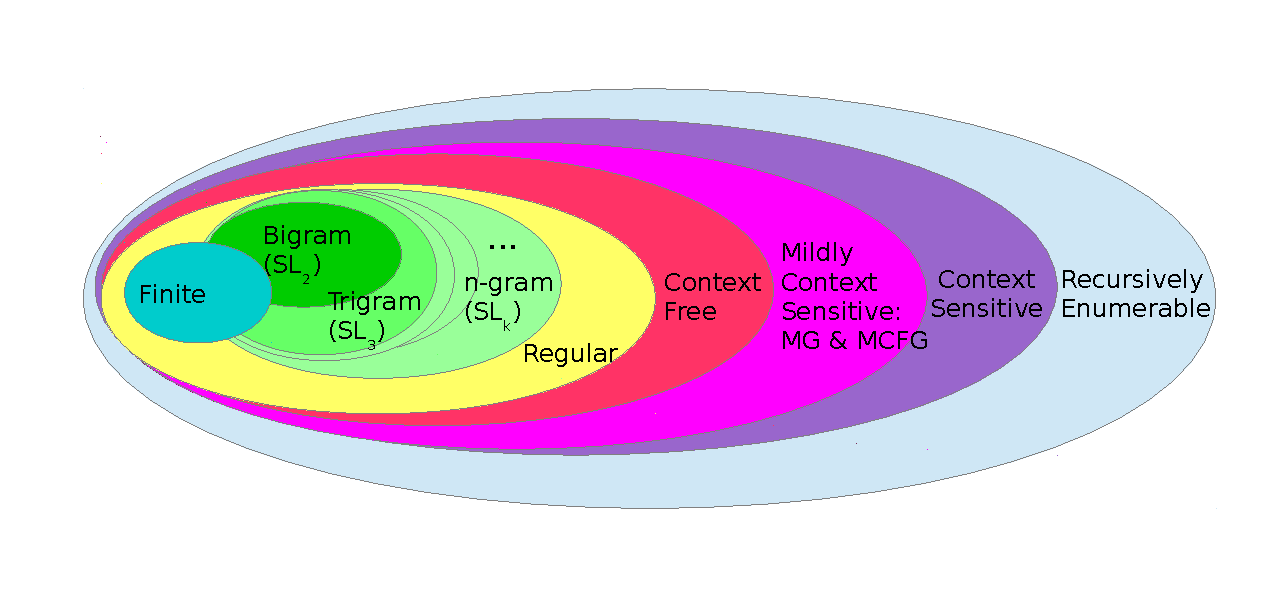
\includegraphics[width=6in]{Chomsky-hierarchy.pdf}

There are certain surface patterns that are known to only be generable with grammars of certain types. For example, $a^nb^n$ famously requires a context free grammar. However, since this is a hierarchy anything you can generate with a lower-level grammar you can also generate with a higher-level grammar. If we have a language or a corpus that is, say, regular, we might still want to say that the grammar that generated it is supra-regular. This would have to be based on either additional facts about the language or corpus, on arguments from parsimony, or on additional information about the source of the corpus. 

In our case we argue from the probability distribution in the corpus. If we have reason to think that the bird generates his song probabilistically, then the probabilities in the grammar predict probabilities in the corpus. A grammar with ``room'' in it to include probabilities for copying should better predict the corpus if the bird is indeed copying.




\subsection{TODO}
\begin{itemize}
\item Prove in a grammar without ambiguity that the algorithm actually moves to the global likelihood maximum.
\item Prove correctness (rule probabilities with the same left hand side sum to one).
\item Prove that each rule update increases the likelihood of the corpus.
\item Prove convergence.
\end{itemize}








\section{Historical and mostly wrong stuff}




Previously we used this update rule:

\begin{definition}[sentence-level update rule]
  Given a sentence $s$ and given a probability assignment $\phi$ we can define an updated probability assignment $\phi'$ as follows:

  $$\phi_s'(q,e,q') = \frac{\sum_{(b,r)\in\PARSES(s)}p_\phi(b,r)~\TC_r(q,e,q')}{\sum_{(b,r)\in\PARSES(s)}p_\phi(b,r)~\SC_r(q)}$$
\end{definition}

%\begin{definition}[sentence-level update rule]
%  Given a sentence $s$ and given a probability assignment $\phi$ we can define an updated probability assignment $\phi'$ as follows:%
%
%  $$\phi_s'(q,e,q') = \sum_{(b,r)\in\PARSES(s)}\frac{p_\phi(b,r)}{\sum_{(b',r')\in\PARSES(s)}p_\phi(b',r')}\frac{\TC_r(q,e,q')}{\SC_r(q)}$$
%\end{definition}

%We can write more simply $p_\phi(s)=\sum_{(b',r')\in\PARSES(s)}p_\phi(b',r')$ so that

%$$\phi_s'(q,e,q') = \frac{1}{p(s)}\sum_{(b,r)\in\PARSES(s)}p(b,r)\frac{\TC_r(q,e,q')}{\SC_r(q)}$$


Similarly, given a corpus, we compute the updates based on all parses in parallel:
\begin{definition}[corpus update rule]
  Given a corpus $C$ and given a probability assignment $\phi$ we can define an updated probability assignment $\phi'$ as follows:

 $$\phi_C'(q,e,q') = \frac{\sum_{s\in C}\sum_{(b,r)\in\PARSES(s)} p_\phi(b,r)~ \TC_r(q,e,q')}{\sum_{s\in C}\sum_{(b,r)\in\PARSES(s)} p_\phi(b,r)~ \SC_r(q)}$$ 
\end{definition}

%Floris' version:
%$$\phi_C'(q,e,q') = \frac{\sum_{s\in C}p(s)\phi_s'(q,e,q')}{\sum_{s\in C}p(s)}$$ 

The sums can't be combined into one sum because sometimes there are parses that visit state $q$ but don't follow transition $(q,e,q')$. However, we still want that visit in the state counts for that transition.

We can't use the probability of the whole corpus because not all sentences have parses that visit all states.



\end{document}


%%% Local Variables:
%%% mode: latex
%%% TeX-master: t
%%% End:
